In order to evaluate the performance of our system we examined the percentage of frames 
correctly classified in a 5-fold cross validation, with our segmentation algorithm, and with perfect segmentation. The perfect segmentation and ground truth label for each frame were determined using the annotation to the development data.

In a noiseless environment (i.e. the 5-fold validation), the system classified events with high accuracy, as can be seen in Figure \ref{fig:kfolds}. However, given perfect segmentation on the development set, our system correctly classified 63\% of frames. This shows that, surprisingly, the input features to the classifier were significantly degraded by noise in the development set. With our segmentation algorithm, the system correctly classified only 36\% of frames. This low accuraccy demonstrates the compounding error of the detection stage.

The confusion matricies of classifier stages of the perfectly segmented events, as well as the events segmented using our algorithm can be seen in Figure \ref{fig:confmat_perfect} and Figure \ref{fig:confmat_seg} respectively.

\begin{figure}[h]
  \centering
  \centerline{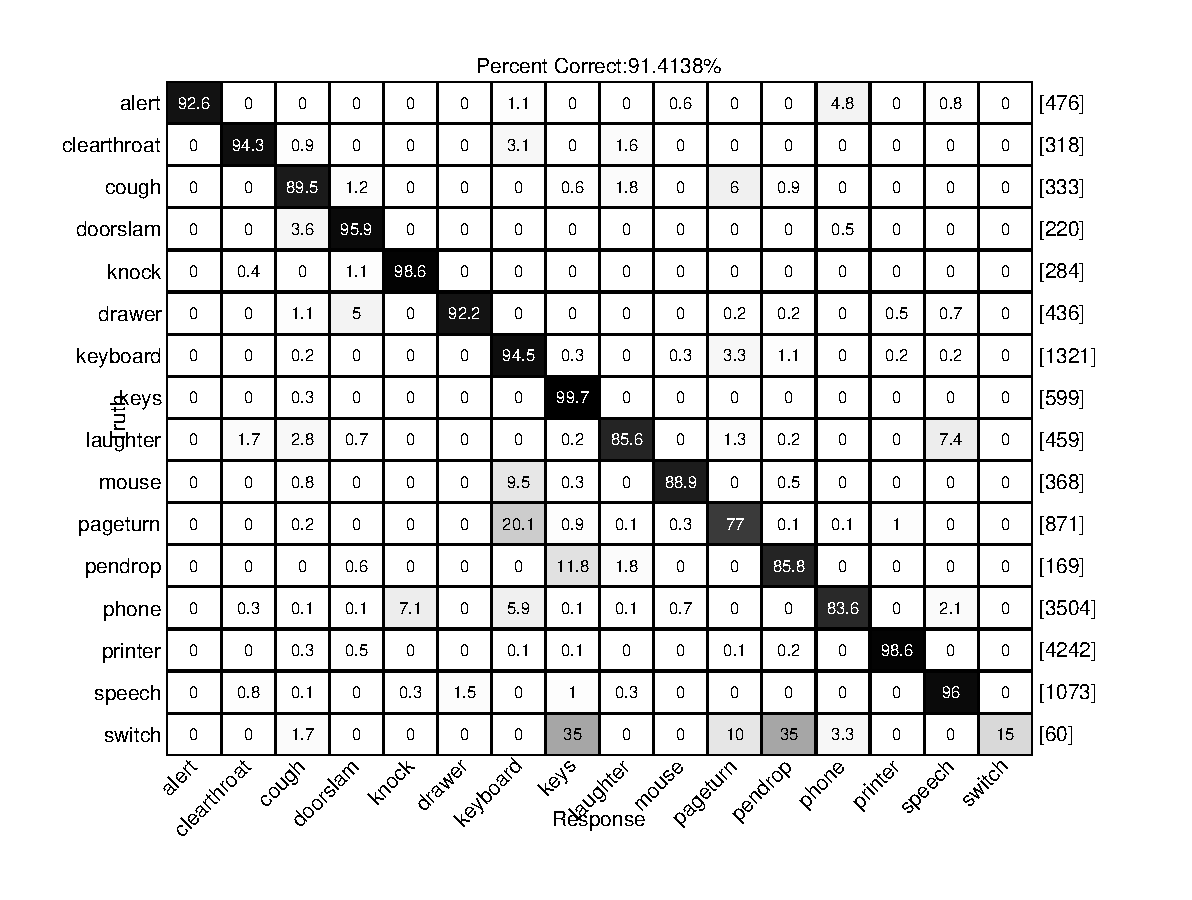
\includegraphics[width=\columnwidth]{kfolds}}
  \caption{Classifier Confusion Matrix with 5-Fold Validation}
  \label{fig:kfolds}
\end{figure}

\begin{figure}[h]
  \centering           \centerline{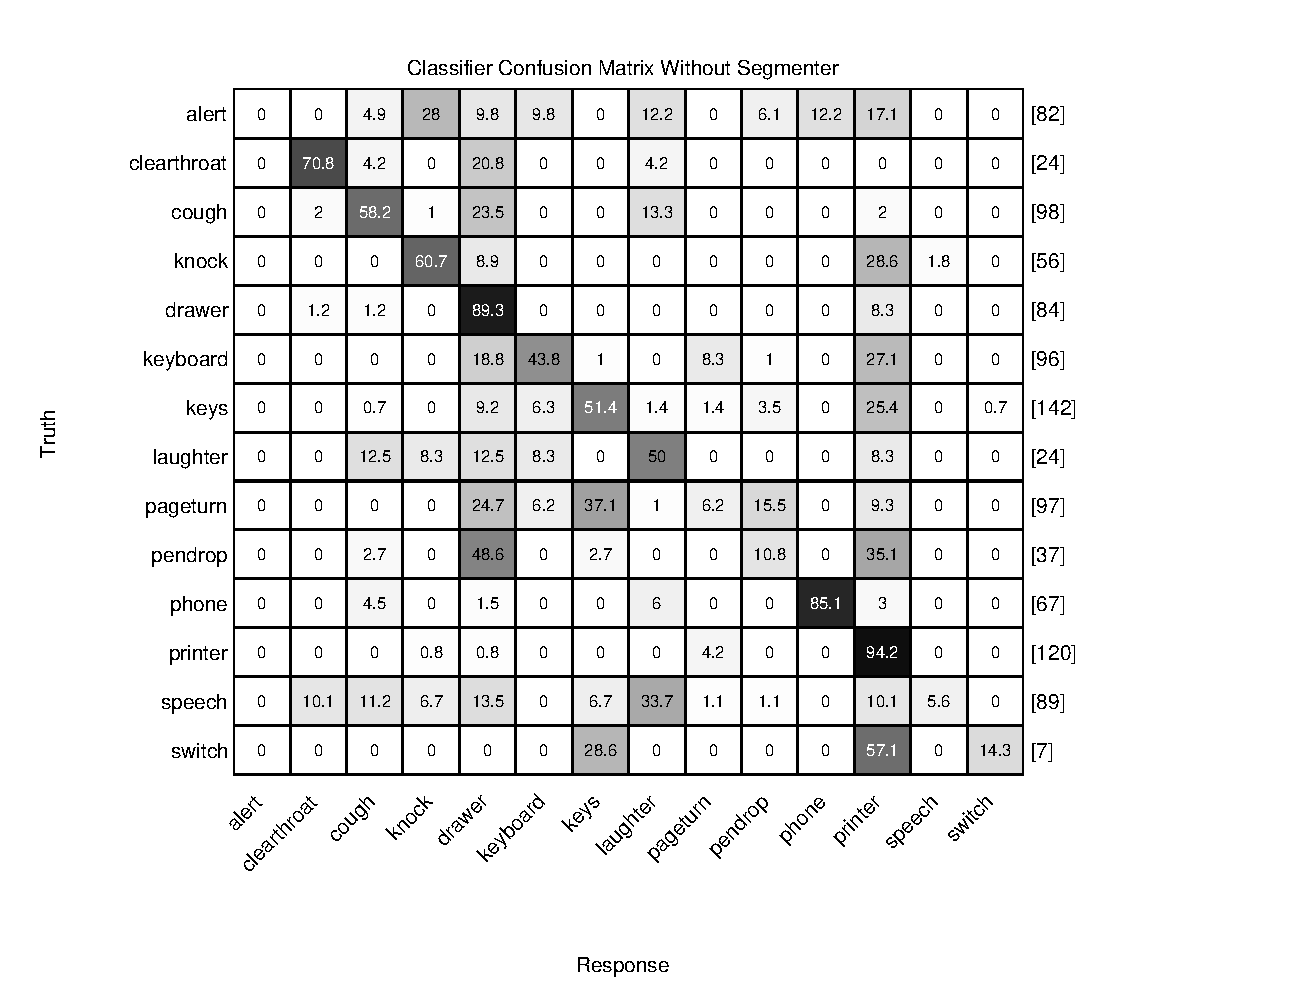
\includegraphics[width=\columnwidth]{confmatrix1}}
  \caption{Classifier Confusion Matrix with ``Perfect'' Segmentation}
  \label{fig:confmat_perfect}
\end{figure}

\begin{figure}[h]
  \centering  \centerline{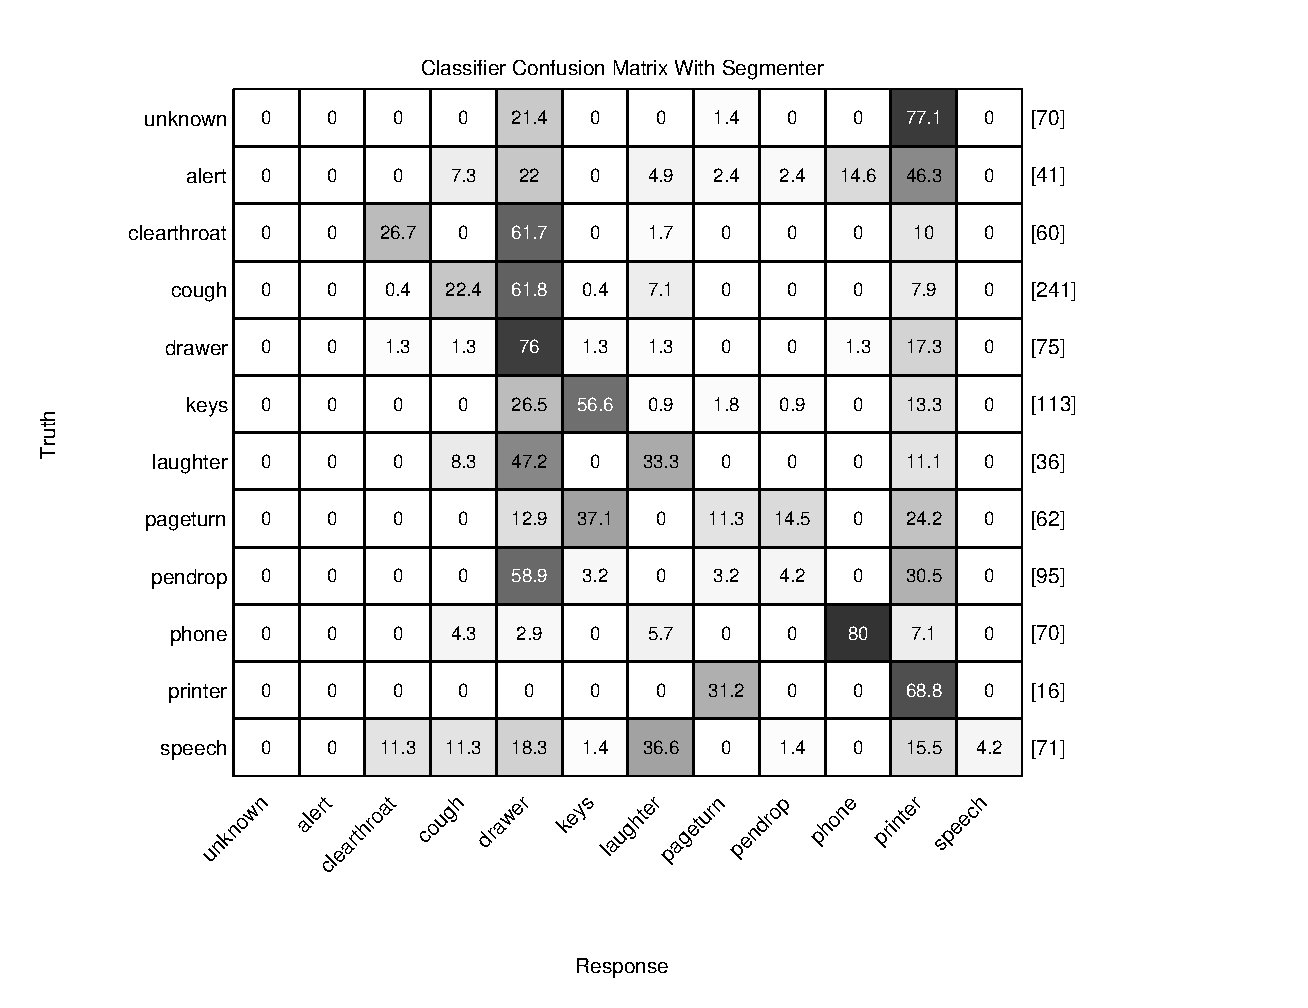
\includegraphics[width=\columnwidth]{confmatrix2}}
  \caption{Classifier Confusion Matrix with Segmenter}
  \label{fig:confmat_seg}
\end{figure}

It is worth noting that the above only hold for frame based classification. Our system was
not able to classify events as well as frames. The class of an event was chosen by taking 
the class chosen most often in the set of frames that formed the event. Because our system
is not able to accurately classify more than 50\% of frames with our segmentation this method
of classifying events does not perform well.  
